
\documentclass[twoside,twocolumn,9pt]{article}
\usepackage{extsizes}
\usepackage[super,sort&compress,comma]{natbib} 
\usepackage[version=3]{mhchem}
\usepackage[left=1.5cm, right=1.5cm, top=1.785cm, bottom=2.0cm]{geometry}
\usepackage{balance}
\usepackage{mathptmx}
\usepackage{sectsty}
\usepackage{graphicx} 
\usepackage{lastpage}
\usepackage[format=plain,justification=justified,singlelinecheck=false,font={stretch=1.125,small,sf},labelfont=bf,labelsep=space]{caption}
\usepackage{float}
\usepackage{fancyhdr}
\usepackage{fnpos}
\usepackage[english]{babel}
\addto{\captionsenglish}{%
  \renewcommand{\refname}{Notes and references}
}
\usepackage{array}
\usepackage{droidsans}
\usepackage{charter}
\usepackage[T1]{fontenc}
\usepackage[dvipsnames]{xcolor}
\usepackage{setspace}
\usepackage[compact]{titlesec}
\usepackage{hyperref}

\usepackage{epstopdf}

\usepackage{amsmath}
\usepackage{amssymb}

% --- Added for this manuscript (theorem environments, tables, figures) ---
\usepackage{amsthm}
\usepackage{booktabs}
\usepackage{siunitx}
\sisetup{detect-weight=true,detect-inline-weight=math}
\usepackage[flushleft]{threeparttable}
\usepackage{tikz}
\usetikzlibrary{positioning,arrows.meta,decorations.pathreplacing}
\graphicspath{{figures/}}

\newtheorem{theorem}{Theorem}
\newtheorem{proposition}[theorem]{Proposition}
\newtheorem{corollary}[theorem]{Corollary}
\newtheorem{definition}{Definition}
\newtheorem{assumption}{Assumption}

% Notation macros shared by the article and the ESI.
\newcommand{\spg}{\mathrm{spg}_\tau}
\newcommand{\Rzero}{R_0}   % true positions / symmetry algorithm on ground truth
\newcommand{\Rone}{R_1}    % render-geometry oracle (the render ceiling)
\newcommand{\RoneRel}{R_1^{0.15}} % the same oracle at the released merge tolerance
\newcommand{\Rtwo}{R_2}    % oracle on a learned detector's output (unscored)
\newcommand{\Rthree}{R_3}  % exact geometry supplied as text
\newcommand{\Rfour}{R_4}   % pixel renders (model perception)
\newcommand{\Symprec}{\mathrm{symprec}}
\newcommand{\PostPerception}[1]{R_1 - R_3(#1)}
\newcommand{\PerceptionComp}[1]{R_3(#1) - R_4(#1)}
\newcommand{\ident}[1]{{\footnotesize\ttfamily #1}}

% Role macros for model arms; identifiers are bound once, in the roster table.
\newcommand{\rlLadder}{the strongest scored model}
\newcommand{\rlWeakest}{the weakest of the fourteen by $R_3$}
\newcommand{\rlFinetuned}{the fine-tuned model arm}
\newcommand{\rlBudget}{the model run at a controlled reasoning budget}
\newcommand{\rlOldGen}{an earlier-generation model}
\newcommand{\rlLadderShort}{Strongest}
\newcommand{\rlWeakestShort}{Weakest}


\definecolor{cream}{RGB}{222,217,201}

\begin{document}

\pagestyle{fancy}
\thispagestyle{plain}
\fancypagestyle{plain}{
\renewcommand{\headrulewidth}{0pt}
}

\makeFNbottom
\makeatletter
\renewcommand\LARGE{\@setfontsize\LARGE{15pt}{17}}
\renewcommand\Large{\@setfontsize\Large{12pt}{14}}
\renewcommand\large{\@setfontsize\large{10pt}{12}}
\renewcommand\footnotesize{\@setfontsize\footnotesize{7pt}{10}}
\makeatother

\renewcommand{\thefootnote}{\fnsymbol{footnote}}
\renewcommand\footnoterule{\vspace*{1pt}% 
\color{cream}\hrule width 3.5in height 0.4pt \color{black}\vspace*{5pt}} 
\setcounter{secnumdepth}{5}

\makeatletter 
\renewcommand\@biblabel[1]{#1}            
\renewcommand\@makefntext[1]% 
{\noindent\makebox[0pt][r]{\@thefnmark\,}#1}
\makeatother 
\renewcommand{\figurename}{\small{Fig.}~}
\sectionfont{\sffamily\Large}
\subsectionfont{\normalsize}
\subsubsectionfont{\bf}
\setstretch{1.125}
\setlength{\skip\footins}{0.8cm}
\setlength{\footnotesep}{0.25cm}
\setlength{\jot}{10pt}
\titlespacing*{\section}{0pt}{4pt}{4pt}
\titlespacing*{\subsection}{0pt}{15pt}{1pt}

\fancyfoot{}
\fancyfoot[LO,RE]{\vspace{-7.1pt}
\includegraphics[height=9pt]{head_foot/LF}}
\fancyfoot[CO]{\vspace{-7.1pt}\hspace{13.2cm}
\includegraphics{head_foot/RF}}
\fancyfoot[CE]{\vspace{-7.2pt}\hspace{-14.2cm}
\includegraphics{head_foot/RF}}
\fancyfoot[RO]{\footnotesize{\sffamily{1--\pageref{LastPage} ~\textbar  \hspace{2pt}\thepage}}}
\fancyfoot[LE]{\footnotesize{\sffamily{\thepage~\textbar\hspace{3.45cm} 1--\pageref{LastPage}}}}
\fancyhead{}
\renewcommand{\headrulewidth}{0pt} 
\renewcommand{\footrulewidth}{0pt}
\setlength{\arrayrulewidth}{1pt}
\setlength{\columnsep}{6.5mm}
\setlength\bibsep{1pt}

\makeatletter 
\newlength{\figrulesep} 
\setlength{\figrulesep}{0.5\textfloatsep} 

\newcommand{\topfigrule}{\vspace*{-1pt}% 
\noindent{\color{cream}\rule[-\figrulesep]{\columnwidth}{1.5pt}} }

\newcommand{\botfigrule}{\vspace*{-2pt}% 
\noindent{\color{cream}\rule[\figrulesep]{\columnwidth}{1.5pt}} }

\newcommand{\dblfigrule}{\vspace*{-1pt}% 
\noindent{\color{cream}\rule[-\figrulesep]{\textwidth}{1.5pt}} }

\makeatother

\twocolumn[
  \begin{@twocolumnfalse}
{
\includegraphics[height=30pt]{head_foot/journal_name}\hfill\raisebox{0pt}[0pt][0pt]{
\includegraphics[height=55pt]{head_foot/RSC_LOGO_CMYK}}\\[1ex]

\includegraphics[width=18.5cm]{head_foot/header_bar}}\par
\vspace{1em}
\sffamily
\begin{tabular}{m{4.5cm} p{13.5cm} }


\includegraphics{head_foot/DOI} & \noindent\LARGE{\textbf{A model-free ceiling for vision--language model evaluation on rendered crystal structures}} \\
\vspace{0.3cm} & \vspace{0.3cm} \\

 & \noindent\large{Can Polat,\textit{$^{a}$} Mustafa Kurban,$^{\ast}$\textit{$^{bc}$} Erchin Serpedin,\textit{$^{a}$} and Hasan Kurban$^{\ast}$\textit{$^{d}$}} \\

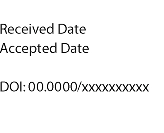
\includegraphics{head_foot/dates} & \noindent\normalsize{A vision--language model that misreads a rendered crystal structure and one that misreasons about it produce the same wrong answer, and every existing method for separating them puts a second model in the loop. When a benchmark is built by rendering a structure whose coordinates are known, no model is needed: inverting the known cameras and re-solving cross-view correspondence returns the answer the images support, a quantity we call the render ceiling. We characterise exactly when that ceiling reaches 1, by an emptiness condition on a set of geometric phantoms, and certify that the condition holds on 2160 structures drawn from the Materials Project, so every point of a model's deficit is attributable to the model. Used as the top rung of an attribution ladder over fourteen vision--language models under a frozen evaluation protocol, the ceiling reverses the prevailing explanation of multimodal failure: supplying exact geometry as text lifts every model but closes the minority of the gap, leaving 13 of 14 limited more by what survives perception than by perception itself. The same instrument catches what a leaderboard cannot: a strong model used as the structure-extraction stage emits syntactically perfect coordinates whose median recall against ground truth is zero, a fabrication downstream accuracy would score as bad reasoning. The construction transfers to any benchmark whose forward rendering is known and invertible, and it returns design rules for benchmark builders: which camera placements are robust to extraction noise, and the tolerance at which a pipeline's own reading, not the images, becomes the binding ceiling.}

\end{tabular}

 \end{@twocolumnfalse} \vspace{0.6cm}

  ]

\renewcommand*\rmdefault{bch}\normalfont\upshape
\rmfamily
\section*{}
\vspace{-1cm}


\footnotetext{\textit{$^{a}$~Department of Electrical and Computer Engineering, Texas A\&M University, College Station, Texas, USA.}}
\footnotetext{\textit{$^{b}$~Department of Prosthetics and Orthotics, Ankara University, Ankara, Turkey.}}
\footnotetext{\textit{$^{c}$~Department of Electrical and Computer Engineering, Texas A\&M University at Qatar, Doha, Qatar.}}
\footnotetext{\textit{$^{d}$~College of Science and Engineering, Hamad Bin Khalifa University, Doha, Qatar.}}
\footnotetext{$^{\ast}$~Corresponding authors. E-mail: kurbanm@ankara.edu.tr; hkurban@hbku.edu.qa}
\footnotetext{\dag~Electronic supplementary information (ESI) available: notation, proofs of the identifiability and scope results, statistical procedures, label-granularity scores, the cell-metric classifier specification, the full render-convention measurements, secondary-axis figures, extended limitations, and the reproducibility record.}

% ORCID iDs (for submission system):
%   Can Polat        0000-0002-1458-302X
%   Erchin Serpedin  0000-0001-9069-770X
%   Mustafa Kurban   0000-0002-7263-0234
%   Hasan Kurban     0000-0003-3142-2866


\section{Introduction}
Vision--language models are entering materials and chemistry workflows as readers of rendered structures,
diffraction data and figures, and benchmarks of that capability now exist for crystal renders and XRD images
alike \citep{xcrys2506,xrdbench2605}. When such a model fails, the remedy depends on where the failure sits:
a perception failure is fixed at the input, in the render protocol or the representation, while a reasoning
failure is fixed in the model. Separating the two requires an independent read of what an image contains,
and for natural photographs that reference does not exist: no procedure recovers a photograph's
information content without invoking a model of some kind. Rendered scientific figures are different. A
ball-and-stick crystal render is an orthographic projection of a structure whose coordinates are known
exactly, under a camera set the experimenter chose, and inverting that projection, by triangulating atom
positions across views and applying a deterministic symmetry algorithm to the reconstruction, returns the
answer the images support with no model at any step. This paper builds that instrument and reports what it
attributes. A two-stage pipeline, which replaces that inversion with a second model, has no model-free row at
all.

\begin{figure*}[t]
\centering
\resizebox{0.92\textwidth}{!}{%
\begin{tikzpicture}[
  font=\small,
  x=8.2cm, y=1cm,
  free/.style={circle, draw=black!70, fill=teal!70!black, inner sep=0pt, minimum size=5.4pt},
  mod/.style={circle, draw=black!70, fill=blue!55!black, inner sep=0pt, minimum size=5.4pt},
  lab/.style={anchor=east, inner sep=1pt},
  sub/.style={anchor=east, inner sep=1pt, black!50, font=\footnotesize},
  val/.style={anchor=west, inner sep=0pt, font=\footnotesize},
  iv/.style={black!45, {|[width=4.5pt]}-{|[width=4.5pt]}},
  ivl/.style={font=\footnotesize, black!55}]

\def\rA{2.10}\def\rB{1.20}\def\rC{0.00}\def\rD{-0.90}
\draw[black!25, dashed] (0.1429,-1.95) -- (0.1429,2.55);
\node[anchor=south, black!45, font=\footnotesize] at (0.1429,2.56) {chance};

\foreach \y in {\rA,\rB,\rC,\rD}{\draw[black!10] (0,\y) -- (1,\y);}

\node[lab] at (-0.03,\rA) {$\Rzero$\ \ true positions};
\node[sub] at (-0.03,\rA-0.36) {symmetry algorithm};
\node[free] at (1,\rA) {}; \node[val] at (1.015,\rA) {1.0000};

\node[lab] at (-0.03,\rB) {$\Rone$\ \ render geometry};
\node[sub] at (-0.03,\rB-0.36) {inversion, then algorithm};
\node[free] at (1.0,\rB) {}; \node[val] at (1.015,\rB) {1.0000};
\node[anchor=east, font=\footnotesize\bfseries, teal!55!black] at (0.9840,\rB) {no model};

\node[lab] at (-0.03,\rC) {$\Rthree$\ \ exact geometry as text};
\node[sub] at (-0.03,\rC-0.36) {model};
\node[mod] at (0.8524,\rC) {}; \node[val] at (1.015,\rC) {0.8524};

\node[lab] at (-0.03,\rD) {$\Rfour$\ \ five renders (pixels)};
\node[sub] at (-0.03,\rD-0.36) {model};
\node[mod] at (0.7333,\rD) {}; \node[val] at (1.015,\rD) {0.7333};

\draw[iv] (0.8524,0.62) -- (1.0,0.62);
\node[ivl, anchor=south] at (0.9262,0.70) {residual 0.1476};
\draw[iv] (0.7333,-1.42) -- (0.8524,-1.42);
\node[ivl, anchor=north] at (0.7929,-1.50) {perception 0.1191};

\draw[black!35] (0,-1.95) -- (1,-1.95);
\foreach \x/\t in {0/0, 0.25/0.25, 0.5/0.50, 0.75/0.75, 1/1.00}{
  \draw[black!35] (\x,-1.95) -- (\x,-2.07);
  \node[anchor=north, black!55, font=\footnotesize] at (\x,-2.09) {\t};}
\node[anchor=north, black!55, font=\footnotesize] at (0.5,-2.44) {crystal-system accuracy};
\end{tikzpicture}}
\caption{The attribution ladder ($n = 210$, $K{=}3$). Each rung answers the same question on the same
structures with one capability removed, and $\Rone$ answers it from the renders' own projection geometry with
no model in the measurement, which is what fixes the top of the ladder. With the extraction tolerance matched
to the symmetry tolerance, $\Rone$ and $\Rzero$ coincide at 1.0000, so the whole 0.2667 the strongest model
leaves is the model's. Model rungs are \rlLadder{} (Section~\ref{sec:roster}).}
\label{fig:teaser}
\end{figure*}

The shape of the argument has prior art. Several studies attribute multimodal failure to perception rather
than inference, whether by converting the image into a model-written description \citep{arc2512} or by
decoupling the two stages in post-training \citep{decouple2605}, but in every prior design we found the
perception stage is itself a model, so the split compares two model configurations, inherits the describer's
errors, and states no quantity for how much of the task the image answers at all. Our separation differs from
those closest in kind on three axes at once: the perception stage is a closed-form inversion rather than a
model or a written description; the reference is an accuracy on the same labels and structures, so it enters
the ladder as a rung; and the split is task-level rather than mechanistic, where attention-masking analyses
locate the layer at which visual access stops mattering \citep{vab2607}. What that buys is a number. Benchmark
headroom is otherwise taken to be one minus the best score, which assumes a ceiling of 1
\citep{zerobench2502}, and assumed ceilings can be wrong by enough to change conclusions
\citep{ceilingart2605}. Where a ceiling is measured rather than assumed, existing practice still puts a model
in it, typically a best-case ensemble over several models' predictions or a hypothetical selector computed
against the labels: an analytical device for what current models can reach rather than a measurement of what
the images contain. The render ceiling is the first such quantity computable with no model anywhere in the
measurement, and it comes with a characterisation of exactly when it is exact (Figure~\ref{fig:teaser}). Here we construct that ceiling, certify the condition under which it is exact, and use it as the top rung of an attribution ladder over fourteen vision-language models. Four contributions follow.

\textbf{(i) Perception is not the bottleneck for most of the roster, once the ceiling is measured.} Used as
the top rung of an attribution ladder on 210 structures under a frozen evaluation protocol, the oracle contradicts
the perception-bottleneck reading it was built to test: with exact geometry supplied as text, the residual
that survives is the larger deficit for 13 of 14 scored models. The single exception ranks second on pixels
and joint-first with exact geometry, so perception dominance is confined to the top of the roster rather than
being a property of the task, which reconciles this result with model-in-the-loop studies that examine
frontier models. We test for a monotone trend across the roster, do not find one at $n=14$, and report the
negative.

\textbf{(ii) A failure a leaderboard cannot see.} A strong model used as the extraction stage emits
syntactically perfect coordinate lists whose median recall against ground truth is 0.0000, a fabrication that
downstream accuracy alone would have scored as bad reasoning and that is detectable only against a model-free
reference.

\textbf{(iii) A characterisation of when a render determines its label, and of what the resulting ceiling
bounds.} Our identifiability result shows the oracle recovers exactly the atoms plus a set of geometric
phantoms, so it never drops an atom and its only failure mode is coincidence. That condition is met here, and
emptiness is a property of the released protocol rather than of the construction, since the same census finds
phantoms once cameras are removed. A companion scope result fixes the reading: the ceiling bounds an
exact-extraction centroid-triangulating pipeline and nothing outside that class. Because $\Rzero$ and $\Rone$
coincide at 1.0000, every point of a model's deficit is attributable to the model.

\textbf{(iv) What a practitioner does with the ceiling: a frontier and a conditioning constant.}
Identifiability being exact, what a practitioner faces is set by the tolerance $\delta$ at which their
extraction stage merges triangulated candidates, and the frontier we trace across $\delta$ says what an
imperfect reader of the same images would lose, which is narrower than what the images withhold. Camera
placement acts through the conditioning constant $\kappa$: fixed in advance for two protocols differing in
cameras alone, it predicted which would be less robust to extraction noise, and we report that prediction with two
that failed. Labels are computed rather than annotated, under a composition-exclusion protocol.

A sceptical reading is that an assumed ceiling of 1 was right all along. Measuring converts that assumption
into a certificate, the certificate fails at two and three views so emptiness is designable rather than given,
and at the merge tolerance our released pipeline used the same oracle reads $\RoneRel = 0.9524$, so an
instrument built on that pipeline alone would have charged 4.8 points of every model's deficit to the
images.

\subsection{Related work}
\label{sec:related}

\textbf{Model-in-the-loop attributions of multimodal failure.} The claim that multimodal failures are
perceptual rather than inferential is argued in several places, always by putting a second model in the loop,
whether as the describer, the decoupled perception stage, or the masked probe of the attribution studies
cited in the introduction. \citet{textoracle2512} serialise the visual stream into
text and conclude that the ceiling is set by the backbone's reasoning; their oracle is a ground-truth
\emph{description}, so it fixes the model's input but leaves the image's information content unmeasured.
\citet{mathlens2510} decompose performance into perception, reasoning and integration on geometry problems
whose diagrams and descriptions come from a common symbolic specification, and find integration dominant;
their perception measure is bundled together with integration rather than isolated. Additional reasoning can
even \emph{reduce} accuracy \citep{dual2509, cotdeg2604}. \citet{vdlm2404} convert raster vector graphics to
SVG with a rule-based encoder before a learned abstraction step; their symbolic stage is still learned, and
none of these designs reports a quantity for how much of the task the image answers on its own.

\textbf{Crystallography with vision--language models.} \citet{xcrys2506} stress-test nine VLMs on rendered
crystal structures under spatial- and com\-po\-si\-tion-exclusion protocols and report that supplying the source
crystallo\-graphic file alongside the image narrows but does not close the gap; the ceiling their gap is read
against is the best observed score rather than a measured bound. \citet{xrdbench2605} benchmark VLMs on XRD
peak indexing, establish that models fail on rendered crystallographic images, and likewise report that
supplying the source file alongside the image fails to close the gap on that target. On the model-free side,
\citet{cryspnet2003} and \citet{extinction2411} predict symmetry from composition and from
diffraction-consistent descriptors respectively, taking chemical or diffraction input rather than an image.
\citet{ziletti2018insightful} classifies crystal symmetry from computed diffraction images with a learned
network, so the reader itself is a trained model rather than a closed-form procedure.

\textbf{Resolution and render protocol.} \citet{resbench2510} and \citet{nativevis2506} show that dynamic
resolution input is a live failure mode for vision-language models. Multi-view correspondence is documented
as a weakness \citep{allangles2504}, and view selection has been optimised through a differentiable renderer
\citep{mvtn2011}, in both cases treating the render or view configuration as something to be learned or
searched rather than analysed for the conditioning it induces.

\textbf{Identifiability from multiple views.} Recovering shape from several orthographic views is classical
\citep{tomasi1992factorization}, and recent work does it with learned self-supervised objectives
\citep{gaussiancad2026}. On the representation-learning side, \citet{daunhawer2023identifiability} give
identifiability guarantees for the latent factors a multi-view contrastive objective recovers; the guarantee
concerns what a learned model recovers rather than exact geometric identifiability of scene content under a
known renderer.

\textbf{Verifying intermediate steps.} \citet{groundscore2603} verify explicit visual premises to make process
reward models reliable, and \citet{cvt2511} add continuous visual tokens for intermediate reasoning; both
treat the intermediate representation as something to be made checkable, without an exact ground-truth
reference against which to check it.

Across these lines, the shared gap is a model-free reference: every design above puts a second model, a
learned encoder, or a searched configuration where a closed-form inversion could stand instead, and none
reports a quantity for how much of the task an image answers on its own. Where the present findings and the
model-in-the-loop attributions overlap, the disagreement is one of measurement rather than finding: exact
geometry closes only a minority of the deficit for 13 of 14 models on the roster used here, and the two
readings are compatible once roster position is conditioned on, since the model-in-the-loop studies above
examine frontier models and the present perception-dominant exception is itself one.

\section{Methods} \label{sec:method} The method has three parts: an oracle that answers the task
with no model in it, the theory that says when it is exact and what it bounds, and the ladder that uses it.

\subsection{Geometric oracle and identifiability}
\label{sec:oracle}

\textbf{Structures and labels.} A crystal structure is a triple $s = (L, X, Z)$ of lattice, fractional
coordinates $X = \{x_i\}_{i=1}^{N}$ and species. The label map $y(s) = \spg(s)$ is the crystal system returned
by a deterministic symmetry algorithm \citep[spglib,][]{spglib2024} at a fixed tolerance $\tau$, so label
correctness is not a competing explanation for model error.

\textbf{Renders.} The frozen protocol renders a $2\times2\times2$ tiling of the conventional cell through five
orthographic cameras $\mathcal{C} = \{c_v\}_{v=1}^{5}$ (three principal-axis, two oblique) at $768$ px. The
tiling is a legibility choice inherited from the convention. Each camera is a known unit direction $d_v$ with
orthographic projection $\Pi_v(p) = P_v\, p$ for a fixed $2\times3$ matrix $P_v$ with orthonormal rows
perpendicular to $d_v$. The task given to a model is: from $(I_1,\dots,I_5)$, name the crystal system.

\textbf{The oracle.} The oracle answers the same question from the renders' own geometry instead of from
pixels: where classical orthographic factorisation estimates the cameras, the render protocol fixes them, so
we invert them in closed form. It forward-projects the ground-truth atom positions of the conventional cell
through each frozen camera, \emph{discards} the correspondence between views, re-solves it by ray intersection
with cross-view verification, and applies $\spg$ to the reconstruction (Algorithm~S1 of the ESI\dag{}). It is
deterministic and CPU-only, and assumes \emph{ideal extraction}: every atom's centroid is available in every view, including
atoms an image hides, so $R_1$ bounds identifiability from the projection geometry rather than from the
pixels, and a visibility-conditioned variant is a separate measurement we have not built.

\textbf{Two tolerances, and why they must be tied.} The oracle carries a tolerance $\delta$ at
which it accepts a ray intersection and merges the resulting candidates, and the label map carries the
symmetry tolerance $\tau$ at which $\spg$ decides. They interact: at $\delta > \tau$ a merge can combine two
distinct atoms and displace the survivor by an amount $\spg$ can see, so the reconstruction is faithful in
atom count yet wrong in symmetry. \emph{The operating rule is therefore to keep $\delta \le \tau$}, and the
identifiability result below assumes exactly this merge. Throughout $\tau = 0.01$\,\AA{}, and every oracle
number is reported with both values stated. Our released pipeline used $\delta = 0.15$\,\AA{}; we write
$\Rone$ for the ceiling in the exact regime $\delta \le \tau$ and $\RoneRel$ for the same oracle read at that
released tolerance (the governing notation is collected in Section~S1 of the ESI\dag{}).

\begin{definition}[Render ceiling] \label{def:ceiling} For an evaluation sample $\mathcal{S}$ under a frozen
protocol $\mathcal{C}$, the \emph{render ceiling} is $\Rone = |\mathcal{S}|^{-1}\sum_{s \in \mathcal{S}}
\mathbf{1}[\,O(s,\mathcal{C}) = y(s)\,]$. \end{definition}

\begin{definition}[Phantom set]
\label{def:phantom}
Fix $\tau \ge 0$. A species-labelled point $(p,z)$ lies in $\Phi_\tau(s,\mathcal{C})$ if it is further than
$\tau$ from every same-species atom, arises as the intersection of the back-projections of two \emph{distinct}
same-species atom images in some pair of views, and projects within $\tau$ of some same-species atom image in
every view. The set depends on $s$ and $\mathcal{C}$ alone; the componentwise statement accompanies the
proofs.
\end{definition}

\begin{theorem}[Soundness and completeness of the oracle]
\label{thm:ident}
Assume at least two directions in $\mathcal{C}$ are linearly independent and distinct same-species atoms are
more than $2\tau$ apart. Then (a) every atom is recovered exactly, by every independent view pair, so the
accepted set contains the atom set $X$ and does not depend on the enumeration order; (b) every accepted
point further than $\tau$ from all same-species atoms lies in $\Phi_\tau(s,\mathcal{C})$, and conversely
every element of $\Phi_\tau(s,\mathcal{C})$ is accepted; and (c) if $\Phi_\tau(s,\mathcal{C}) = \emptyset$
then merging accepted points at tolerance $\tau$ returns exactly $X$, hence $O(s,\mathcal{C}) = y(s)$.
\end{theorem}

Proofs are in Section~S2 of the ESI\dag{}. Parts (a) and (b) say the oracle has no failure mode other than
$\Phi_\tau$: exact on the atoms, and everything it can get wrong is a coincidence fixed by the structure and
cameras. The separation hypothesis in (c) is not cosmetic, and the statement does not lift to labels, since a
reconstruction containing a phantom may still return $y(s)$.

The hypothesis of (c) is satisfied on this benchmark rather than assumed: a direct census of $\Phi_0$ finds
it empty on every certified structure under the released five-camera protocol, and nonempty once cameras are
removed, so $\Rone = 1.0000$ whenever $\delta \le \tau$ and emptiness is a property of the protocol rather
than of the construction. That census is why we treat identifiability as exact and place the operational
degradation in the extraction tolerance instead.

\begin{proposition}[What the ceiling bounds, and what it does not]
\label{prop:scope}
Let $\kappa = \max_{v \neq w} \|[P_v; P_w]^{+}\|_2$ over the enumerated independent view pairs. Call a
procedure a \emph{centroid-triangulating pipeline} if it extracts species-labelled 2D centroids per view
with error at most $\varepsilon$, triangulates at tolerance $\tau$, and applies $\spg$. At
$\varepsilon = 0$ it returns $O(s,\mathcal{C})$ on every structure, so its accuracy is exactly $R_1$; for
$\varepsilon > 0$ the same holds on every structure none of whose compared distances lies within
$2\kappa\varepsilon$ of $\tau$.
\end{proposition}

The constant is a property of the camera set, $\kappa = 2.7321$ here, and it diverges as two directions
approach parallel, so a protocol of nearly collinear cameras has a ceiling that is fragile to extraction error
even when it is high. Because identifiability here is exact, that fragility is the whole of what distinguishes
protocols on this benchmark, and $\kappa$ is used to
predict it in advance rather than to explain it afterwards. The proposition licenses reading $R_1$ as a
ceiling and fixes the limits: it covers no procedure using shading, occlusion ordering or bond rendering, and
no model that answers without reconstructing. Its band is sufficient for label agreement rather than tight,
which we test empirically.

Two design consequences follow (Corollary~S1 of the ESI\dag{}): adding a view can never destroy identifiability,
and a camera aligned with a lattice vector separates no atoms differing by multiples of it.

Part (b) constrains a single camera and with five it does not bind, so tiling is not an identifiability
question on this protocol but a conditioning one. We prove no rate for how $\Phi_\tau$ grows with atoms per
cell, since the natural union bound needs generic positions and crystal atoms sit on special positions; that
dependence is measured instead and reported as a decomposition.

\subsection{The attribution ladder}
\label{sec:ladder}

\begin{definition}[Rungs and shares]
\label{def:ladder}
For a model $m$ evaluated on the same structures, let
$\Rzero = \tfrac{1}{n}\sum \mathbf{1}[\spg(s) = y(s)]$ (the symmetry algorithm on ground-truth positions),
$\Rone$ the oracle ceiling of Definition~\ref{def:ceiling},
$\Rthree(m)$ the accuracy of $m$ given ground-truth fractional coordinates, species and cell parameters as
text, and
$\Rfour(m)$ the accuracy of $m$ on the pixel renders. Define the \emph{perception component}
$P(m) = \PerceptionComp{m}$, the \emph{post-perception residual} (elsewhere the \emph{symbolic residual})
$S(m) = \PostPerception{m}$, and the \emph{perception share} $P(m) / (R_1 - R_4(m))$. $\Rtwo$ denotes the oracle run
on a learned detector's output.
\end{definition}

$R_1 - R_4(m)$ is a model's total deficit against a model-free reference, $P(m)$ the slice closed by supplying
perception's output as text, and $S(m)$ the slice that supplying it does not close. Because $R_1$ carries no
model in its own measurement, the split is a subtraction against a fixed, certified quantity rather than
against a second model's output. Three conditions make the shares interpretable: the rungs are scored on the
same structures with all comparisons paired; $R_3$ and $R_4$ share a decode budget; and $S(m)$ bounds rather
than isolates symmetry reasoning, a bound we test below and which the test does not clear. Referencing to
$R_1$ rather than $R_0$ costs nothing here, since $\Rzero = \Rone = 1.0000$ and the shares in
Table~\ref{tab:rungs} need no correction; at $\RoneRel$ the two rungs differ by $0.0476$ and every share
would shift downward, which is one practical reason to tie $\delta$ to $\tau$. Note that $R_4$ enters both
numerator and denominator, so the share cannot vary independently of pixel accuracy.

\begin{table*}[t]
\centering
\caption{The attribution ladder ($n = 210$, $K{=}3$). \rlLadderShort{} and \rlWeakestShort{} are
\rlLadder{} and \rlWeakest{}, chosen to span the range. Every derived quantity is a difference of rows above
it. $\Rzero$ is definitional: the label \emph{is} the algorithm applied to the structure. $\Rone$ is
measured, and equal to $\Rzero$: with the extraction tolerance tied to the symmetry tolerance the phantom set
is empty on all 210 structures and the oracle returns every label, so the render protocol withholds nothing
and the entire deficit below is the model's; read at the released merge tolerance this row is
$\RoneRel = 0.9524$. $\Rtwo$, the oracle on a learned detector's output, is unscored under a pre-registered
triangulation-failure gate.}
\label{tab:rungs}
\footnotesize
\setlength{\tabcolsep}{4pt}
\begin{tabular*}{\textwidth}{@{\extracolsep{\fill}}ll S[table-format=1.4] S[table-format=1.4]@{}}
\toprule
& & \multicolumn{2}{c}{Accuracy} \\
\cmidrule(l){3-4}
Rung & Reader & {\small \rlLadderShort} & {\small \rlWeakestShort} \\
\midrule
\multicolumn{4}{@{}l}{\emph{Model-free}} \\
\quad $\Rzero$\; true positions        & symmetry algorithm      & \multicolumn{2}{c}{1.0000} \\
\quad $\Rone$\; render geometry       & inversion, then algorithm & \multicolumn{2}{c}{1.0000} \\[1pt]
\multicolumn{4}{@{}l}{\emph{Model}} \\
\quad $\Rthree$\; exact geometry as text & model                  & 0.8524 & 0.4143 \\
\quad $\Rfour$\; five renders (pixels)  & model                  & 0.7333 & 0.3667 \\
\midrule
\multicolumn{4}{@{}l}{\emph{Derived} (Definition~\ref{def:ladder})} \\
\quad perception component $\Rthree{-}\Rfour$        & & 0.1191 & 0.0476 \\
\quad post-perception residual $\Rone{-}\Rthree$    & & 0.1476 & 0.5857 \\
\quad perception share $P/(P+S)$              & & \bfseries 0.4466 & \bfseries 0.0752 \\
\bottomrule
\end{tabular*}
\end{table*}

\subsection{Benchmark construction}
\label{sec:benchmark}

\textbf{Certified labels.} Each structure's crystal system, Bravais lattice, point group and space group
are derived from its coordinates by $\spg$ at the canonical tolerance ($\Symprec=0.01$, angle
tolerance $5^\circ$), with a tolerance sweep that quarantines any structure whose space group is not stable
across it. On a separate stratified sample disjoint from training and evaluation, our labels agree with the
source-database space group in $220/220$ cases (one-sided exact 95\% lower bound $0.9865$; sampling detail in
Section~S3 of the ESI\dag{}). This is not a check against an independent symmetry-detection method: both source
databases derive their space groups through the same spglib library used here, so this certifies
tolerance-consistency within one algorithm family rather than agreement between distinct algorithms.

\textbf{Source structures.} Structures are drawn from the Materials Project \citep{jain2013commentary} as conventional-cell CIFs under
a composition-exclusion split reserving 13 elements for evaluation only. The released 1,820 structures (1,610 train / 210 eval) have zero
train/eval/prior leakage, under the Materials Project's CC~BY~4.0 licence; the database snapshot is not
recorded.

\textbf{Composition exclusion.} No chemical composition in any evaluation set appears in training. Without
this, symmetry is partly predictable from composition alone, and a model could score well without reading the
image.

\textbf{Label granularity.} The crystal system is the headline label, but the same reconstruction determines
the Bravais lattice, point group and space group, so neither the identifiability result nor the ceiling is
specific to the seven-way target; Section~S4 of the ESI\dag{} scores all four.

\section{Results and discussion} \label{sec:experiments} We report the ceiling and the ceiling-to-model gap,
then the design consequences, then the controls that decide what the gap may be attributed to.
\subsection{Model roster}
\label{sec:roster}
Main text names every model arm by role rather than by vendor identifier (Section~\ref{sec:method}); this
subsection binds each role to its identifier, run conditions, and the accuracies attached to it elsewhere in
the paper, and is the reference for contributions (i) and (ii).
Table~\ref{tab:roster} gives the binding: for each role, the exact identifier, the condition(s) it was run
under, its sample and decode budget, and the accuracies attached to it elsewhere in the paper. The
supervised reference arm discussed alongside \rlFinetuned{} shares the same base model but differs in
training recipe, and is bound on that basis rather than treated as a separate vendor model.

\begin{table*}[t]
\centering
\caption{Role-label roster. Every accuracy figure here is reported elsewhere in the paper under the same
role label; this table adds only the vendor identifier and the run conditions. \rlLadderShort{} and
\rlWeakestShort{} are the short forms used in the columns of Table~\ref{tab:rungs}.}
\label{tab:roster}
\small
\begin{tabular*}{\textwidth}{@{\extracolsep{\fill}}>{\raggedright\arraybackslash}p{0.17\textwidth}>{\raggedright\arraybackslash}p{0.21\textwidth}>{\raggedright\arraybackslash}p{0.27\textwidth}>{\raggedright\arraybackslash}p{0.25\textwidth}@{}}
\toprule
Role label & Identifier & Conditions and sample & Accuracies \\
\midrule
\rlLadder{} (\rlLadderShort) & \ident{gemini-\allowbreak 3.6-\allowbreak flash} & Ladder ($\Rzero$/$\Rone$/$\Rthree$/$\Rfour$), $n{=}210$, $K{=}3$; also the newer arm in the one-generation comparison (same model, same label, not a second arm) &
$\Rzero{=}1.0000$; $\Rone{=}1.0000$; $\Rthree{=}0.8524$; $\Rfour{=}0.7333$; closes 54.1\% of its generational headroom, computed against $\RoneRel$ \\
\rlWeakest{} (\rlWeakestShort) & \ident{gpt-\allowbreak 4.1-\allowbreak mini} & Coordinate condition ($\Rthree$/$\Rfour$), $n{=}210$, $K{=}3$ &
$\Rthree{=}0.4143$ (minimum of the 14 scored); $\Rfour{=}0.3667$ \\
\rlFinetuned{} & \ident{Qwen/\allowbreak Qwen3-\allowbreak VL-\allowbreak 8B-\allowbreak Instruct} & Supervised-then-GRPO, single seed; $n{=}210$; headline at $K{=}8$, also reported at $K{=}3$ &
$0.6905$ at $K{=}8$; $139/210{=}0.6619$ at $K{=}3$; model side of the ceiling-to-model gap (discordance $61{:}6$, $p{=}1.5\times10^{-12}$) \\
Supervised reference arm & \ident{Qwen/\allowbreak Qwen3-\allowbreak VL-\allowbreak 8B-\allowbreak Instruct} (same base as \rlFinetuned{}, supervised-only recipe, no GRPO) & Supervised LoRA, three seeds, 416\,px, 1{,}610 training examples, no augmentation &
Mean $0.6143$ (SD $0.0515$); per-seed $0.590 / 0.567 / 0.686$ \\
\rlBudget{} & \ident{claude-\allowbreak opus-\allowbreak 5} & Two reasoning-budget settings (minimal, provider default), $n{=}210$, $K{=}3$ &
$130/210{=}0.6190$ under both settings; $169/210$ agreement, discordance split $13{:}13$, $p{=}1.0000$ \\
\rlOldGen{} & \ident{gemini-\allowbreak 2.5-\allowbreak flash} & Zero-shot leaderboard, $n{=}210$, $K{=}3$ &
Leaderboard best row $0.4429$; closes 64.0\% of its generational headroom, computed against $\RoneRel$ \\
\bottomrule
\end{tabular*}
\end{table*}

\textbf{Roster composition by condition.} The zero-shot leaderboard scored 13 of a pre-registered 14; the
image-removal control scored 13 of 16; the coordinate condition scored 14 of 15. Every exclusion is a
pre-registered API-error, parse or endpoint gate, and every unscored entry is reported unscored rather than
dropped.

\textbf{Protocol detail: composition-exclusion split.} The random seed fixing the composition-exclusion
split of Section~\ref{sec:benchmark} is 23. The 13 elements reserved for evaluation only are Cd, Ce, Hg, In,
Ir, La, Mn, Os, Re, Ru, Tc, Ti and Tl.

The zero-shot leaderboard behind the headline gap is given in Figure~\ref{fig:leaderboard}; the remaining
secondary-axis figures are in Section~S7 of the ESI\dag{}.

\begin{figure*}[t]
\centering

\includegraphics[width=0.92\textwidth]{figures/leaderboard.pdf}
\caption{No scored model reaches half the oracle's 1.0000 on the original sample. Zero-shot crystal-system
accuracy, $n=210$, $K=3$, 13 models across eight vendors. Solid line: the shape-free baseline on this sample,
0.5286; dashed line: seven-way chance, 0.1429. Error bars: measured run-to-run spread of $K{=}3$ majority
voting, a mean of 5.0 of 210 structures across two sweep runs. Every model on this draw falls below the
shape-free baseline; that pattern is specific to this draw and does not hold at $n = 1933$
(Section~\ref{sec:controls}).}
\label{fig:leaderboard}
\end{figure*}

\subsection{Main results}
\label{sec:results}

\textbf{Rosters.} The three conditions score overlapping but non-identical model sets. The 13 scored zero-shot
models ran on the frozen protocol with a verbatim prompt and no per-model tuning; the best reaches
$93/210 = 0.4429$, far below the oracle's 1.0000. A cell-metric random forest, whose feature specification and
reading sensitivity are detailed in Section~S5 of the ESI\dag{}, reaches 0.8952 on the same label,
above every model, which reproduces an established capability rather than contributing one and is not
comparable to composition-only predictors, since it reads cell geometry rather than chemical composition.

The 0.6905 fine-tuned figure is a single-seed supervised-then-GRPO run at $K{=}8$, distinct from the strongest
zero-shot $R_4$ of 0.7333 on the ladder, and it sits inside the supervised reference arm's across-seed spread,
so \emph{we make no claim that it improves on that arm}; it is used only as the model side of the
ceiling-to-model gap, which survives any seed in that spread.

\subsection{Perception versus the post-perception residual}
\label{sec:residual}

\textbf{Perception dominance is a property of the top of the roster, not of the task.} Supplying ground-truth
geometry as text, the CIF-supplied condition introduced in Related Work and used here as prior methodology,
lifts every model substantially, and none reaches the oracle: the best is 0.8524 against 1.0000
(Figure~\ref{fig:ladder}). The
pre-registered decomposition of Definition~\ref{def:ladder} gives a median perception share of 29.0\% across
the 14 models scored under the coordinate condition (bootstrap 95\% CI $[0.149, 0.358]$), with the
post-perception residual the larger of the two for 13 of them ($p = 0.0018$); the two columns of
Table~\ref{tab:rungs} differ in share by a factor of 5.9. The single exception is the model with the
second-highest $R_4$, tied first on $R_3$, which is why studies confined to frontier models see perception
dominate: their sample sits inside the one region of the roster where it does. Because
$\Rone = \Rzero = 1.0000$ these shares need no reference correction; read against $\RoneRel$ the same
decomposition gives 12 of 14 ($p = 0.0129$), so the conclusion holds at either point of the frontier.

The natural strengthening, that the share rises with model strength, is \emph{not} supported: across the
14 models the share and pixel accuracy are unrelated (Spearman $\rho = -0.1588$, $p = 0.5877$), and we report
the negative rather than the ordering. The raw component moves the other way, $R_3 - R_4$ correlating with
$R_4$ at $\rho = -0.6439$, so the strongest pixel performers are those for whom exact geometry adds least
even though the \emph{share} it closes shows no trend.

\begin{figure*}[t]
\centering

\includegraphics[width=0.92\textwidth]{figures/ladder.pdf}
\caption{Exact geometry as text lifts every model and none reaches the oracle, and the share it closes
tracks no trend in pixel accuracy. Marker shape and colour identify the model in both panels (key below).
(a) Per-model $\Rfour$ (pixels, open marker) and $\Rthree$ (exact geometry as text, filled marker) on the
original evaluation sample ($n=210$, $K=3$), rungs as in Definition~\ref{def:ladder}, with the $\Rone$
oracle at 1.0000 and seven-way chance drawn; $\Rtwo$ is omitted (unscored under its pre-registered gate).
(b) Perception share of the deficit against $\Rfour$: 13 of the 14 models fall below the parity line, so the
deficit that survives exact geometry is the larger one for most of the roster, and the share tracks no trend
in pixel accuracy (Spearman $\rho = -0.1588$, $p = 0.5877$). Shares, the median 0.2901 and its bootstrap
95\% CI $[0.1492, 0.3576]$ (band) are computed against the exact ceiling $\Rone = 1.0000$.}
\label{fig:ladder}
\end{figure*}

\textbf{A control pair makes $R_3$ readable.} The same prompt carrying the chemical formula alone collapses
every scored model toward chance, while with full geometry substituted for images every model reaches between
0.4143 and 0.8524, so the lift is the geometry rather than text-mode prompting.

\subsection{The ceiling is exact; the frontier is in extraction tolerance}
\label{sec:frontier}

\textbf{Identifiability is exact.} Enumerating the phantom set over all ten independent view pairs finds
$\Phi_0 = \emptyset$ on every one of the 2160 certified structures under the released five-camera protocol,
and the oracle returns the correct label for all of them, reconstructing positions to
$3.9\times10^{-15}$\,\AA{} with no atom dropped and no phantom accepted. So $\Rone = 1.0000$ on both samples
at any $\delta \le \tau$, and the hypothesis of Theorem~\ref{thm:ident}(c) is met rather than assumed.
Emptiness is a property of the protocol and not of the construction: the same census over camera subsets
leaves $\Phi_0$ nonempty on 15.4\% of two-view subset-structure pairs and 1.9\% of three-view pairs, so the
fifth camera is doing real work.

\textbf{What degrades is the extraction stage.} A practitioner does not have exact centroids, and the merge
tolerance $\delta$ is the parameter that matters. Reading the same oracle across $\delta$ at fixed $\tau$
traces a frontier: 1.0000 at $\delta \le \tau$, 0.9810 at $5\tau$, and
$\RoneRel = 0.9524$ at the released $15\tau$, with $0.8785$ there on the scaled sample. The loss is entirely
over-merging rather than coincidence, since every structure it costs recovers the correct atom count and has
its closest same-species pair at more than eleven times $\delta$.

This relocates the quantity a reader should treat as the ceiling: identifiability from the renders is total,
and what an actual pipeline achieves is a property of its extraction stage. Every ceiling-to-model gap below
is wider under this reading than at the released tolerance, so no comparison depends on which point of the
frontier is chosen.

\subsection{Controls and intermediate verification}
\label{sec:controls}

\textbf{The residual is an upper bound, and we tested it.} It may include long-list handling rather than
symmetry reasoning: regressing per-structure $R_3$ correctness on atom count, 13 of 14 models show a negative
association ($p=0.0018$) that is not symmetry difficulty in disguise, so $S(m)$
bounds a symmetry-reasoning deficit rather than measuring one.

\textbf{A learned extractor fabricates its output.} Substituting a strong model as the extraction stage,
prompted for species and positions with the symmetry question withheld, then having a weaker model answer from
that text, yields exactly the majority stratum's base rate, so downstream accuracy measures nothing. The
informative measurement is the intermediate, scored against ground truth: median recall 0.0000, with 105 of
206 structures having not one emitted atom within tolerance of a real one despite a median of 48 well-formed
atoms each, where a connected-component blob detector reaches 0.400 on the same task. \emph{A two-stage
pipeline whose intermediate cannot be checked will
attribute fabrication to reasoning}, and only a model-free reference distinguishes the two.

\textbf{The models use the image, and have not memorised the answer.} We ran an image-absent control, the
identical prompt carrying the chemical formula and no renders, which is also the control pair that makes
$R_3$ readable in Section~\ref{sec:residual}. Every scored model collapses toward
chance (mean 0.1487 against 0.1429) and the paired difference is significant for 10 of 13, the three nulls
being the three weakest models. This also bounds pretraining
contamination, which composition exclusion does not: a model that had memorised composition-to-symmetry
mappings would beat chance on the formula alone, and none does.

\textbf{Image-removal control, per model.} Figure~\ref{fig:noimage} gives the per-model breakdown: each model answered the identical prompt with the five
renders and with the chemical formula alone, and the paired difference is significant for 10 of the 13
scored, the three nulls being the three weakest models.


\begin{figure*}[t]
\centering

\includegraphics[width=0.92\textwidth]{figures/noimage.pdf}
\caption{Removing the image collapses every model toward chance. Each model answered the identical prompt
with the five renders and with the chemical formula alone, paired per structure (original sample, $n=210$,
$K=3$, 13 scored of 16 attempted); model identifiers are drawn at the end of each bar pair. Stars mark
models whose paired difference is significant, 10 of the 13, the three nulls being the three weakest models
(two of which are at chance even with images); the dashed line is seven-way chance.}
\label{fig:noimage}
\end{figure*}

\textbf{A below-baseline comparison is scoped to its sample, and does not survive scale-up.} On the
original sample every model falls below a shape-free baseline reading only atom count, density and cell
volume (0.4429 against 0.5286, one-sided $p = 0.0078$), but a larger set at $n = 1933$ generated under
identical rules puts that baseline at 0.2054, so \emph{the 0.5286 is a property of the original draw, not of
the task}. The same size-matched control shows the oracle's apparent drop at scale \emph{is} a cell-size
effect, 0.8774 on the full sample against 0.9459 at matched cell size, since more atoms per cell means more
candidate coincidences of the kind Definition~\ref{def:phantom} counts. The ceiling-to-model gap therefore
survives scale-up while the baseline comparison does not.

\textbf{What the controls do and do not isolate.} Three competing explanations for the gap are excluded by
design: that the renders lack the answer, by $R_1$ and the occluder classification; that models pattern-match
or have memorised the label, by the image-removal control; that the $R_3$ lift is text mode rather than
geometry, by the formula-only arm. Two are not excluded: the residual is an upper bound, and the extraction
share is bounded from neither side. A second execution of the
sweep differs by 5.0 structures on average, so adjacent leaderboard rows are not separable.

\subsection{Render conventions}
\label{sec:conventions}

At exact extraction the frozen protocol, the off-axis camera perturbation and the released tiled geometry
each return all 210 labels, so no camera choice in this family withholds any part of the task; what separates
them is conditioning. Before measuring we fixed $\kappa = 2.7321$ for the frozen cameras and
$\kappa = 8.4258$ for the off-axis perturbation, predicted that the more poorly conditioned protocol would
tolerate proportionally less centroid error, and recorded a noise budget from the band of
Proposition~\ref{prop:scope}. Injecting per-view Gaussian centroid noise returns one confirmation and two
failures, and we report all three. The prediction that held is the one that isolates $\kappa$: frozen and
off-axis differ in camera placement alone, and the frozen protocol tolerates $2.1\times$ the noise, with
paired comparison separating them at $\sigma = 0.02$\,\AA{} (102 structures against 2,
$p = 5.4\times10^{-28}$). Two predictions failed, the three-way ordering including the tiled arm and the
absolute noise budget, the latter optimistic by a factor of 31 because the band is sufficient rather than
tight. So $\kappa$ orders protocols differing only in cameras and delivers neither a usable noise budget nor a
cross-density ordering; stating both is the point of fixing the prediction first. View count behaves as
Corollary~S1(a) of the ESI\dag{} says, and what the protocol withholds through occlusion remains under 1\% of
atoms and changes no classification. The noise grid, both failure mechanisms, per-pair $\kappa$ values, the
density decomposition and the probe power analysis are in Section~S6 of the ESI\dag{}.

\textbf{Occluder classification.} This is the occlusion audit referenced in Section~\ref{sec:controls}.
Because the oracle assumes ideal extraction, occluders in the released
renders were classified by whether each one hides a symmetry-equivalent copy of the atom it occludes; most
occlusion hides nothing recoverable, and since triangulation needs only two clear views this holds for
under 1\% of atoms (0.26\% and 0.87\% of the two samples) even before classification. The redundant-only
control removes only occluders in that recoverable class, leaving informative occlusion untouched.
Figure~\ref{fig:conditions} reports recovery under all three conditions on both evaluation samples.

\begin{figure*}[t]
\centering

\includegraphics[width=0.92\textwidth]{figures/conditions.pdf}
\caption{Removing informative occlusion from the oracle's input changes no classification, so what the
renders hide is small and redundant, and the removals do reach the reconstructor. Expansion sample,
$n = 210$, four views. (a) Symmetry recovery under the four occlusion conditions: O0 unconditioned, O1
informative occluders removed, O2 all occluders removed, O3 the pre-registered random-removal control; the
dashed line is O0. (b) Exact atom-count match under the same conditions, which moves across them, so the
flat recovery in (a) is a property of what occlusion hides rather than a failure of the intervention to
reach the reconstructor.}
\label{fig:conditions}
\end{figure*}

\subsection{Limitations and scope}
\label{sec:limits}
 The construction needs a known, invertible
forward rendering, which holds for procedurally generated benchmarks generally but is instantiated here on one
task in one domain, so what is not shown is that a second instantiation reproduces the same qualitative
findings; it does not depend on orthography as heavily as the algebra suggests, since under calibrated
perspective Theorem~\ref{thm:ident} survives while Corollary~S1(b) of the ESI\dag{} fails and $\kappa$ becomes
position-dependent. The oracle assumes ideal extraction, so $R_1$ bounds what is recoverable rather than what
is achievable, and the one extractor evaluated end to end fails the hypothesis of
Proposition~\ref{prop:scope} on soundness, completeness and localisation together; a visibility-conditioned
variant is a distinct measurement we have not built, and no human baseline exists. Because $\Phi_0$ is empty
here, identifiability contributes nothing to the ceiling-to-model gap, which sharpens the instrument but means
the single headline number a reader might want does not exist: what exists is the frontier plus the
class-membership statement of Proposition~\ref{prop:scope}, and $\kappa$ governs one axis of that frontier
only, so it is a design comparator rather than a tolerance budget. Finally, the labels are computed rather
than annotated, but the databases they are cross-checked against derive their own assignments through the same
library (Section~\ref{sec:benchmark}), so certification establishes stability within one algorithm family
rather than agreement between distinct ones; the rosters carry no current-frontier arm beyond the three
compared and no prompt-sensitivity sweep was run, the remaining secondary-axis findings are collected in
Section~S7 of the ESI\dag{}, $R_3$ used a single textual schema, and the model arms were not
re-run at $n=1933$, so that gap is bounded on the oracle side only. Each limit is given in full in
Section~S8 of the ESI\dag{}.

An oracle that recovers structure from a render measures information, not scientific competence, and a
ceiling reported here should not be read as evidence that a model, or a person, can solve the underlying
task. Every ceiling in this article is reported with the tolerance at which it was read, so no number can be
quoted without the regime that produced it, and the per-structure prediction vectors are released so any
ceiling can be re-derived rather than cited.


\section{Conclusions}
A multimodal benchmark built by rendering a known object has a measurable ceiling, computable without a model
and without putting a second model in the loop, and the condition under which it reaches 1 can be stated
exactly. That condition holds here, so what an imperfect reader loses is a frontier in extraction tolerance
rather than a limit of the images. Applied to the roster the ceiling contradicts the reading it was built to
test: exact geometry leaves most models limited by what remains once perception is removed, perception
dominance is confined to the strongest models, and a learned extraction stage can fabricate its output while
staying syntactically perfect. The method transfers to any modality whose forward rendering is known and
invertible, rendered molecular conformers, protein structure renders, and any figure plotted from known
numerical data admitting the same model-free ceiling, and measuring it before a benchmark is released tells
its builder whether the images ask the question the labels answer.


\section*{Author contributions}
C.P.: methodology, software, formal analysis, visualization, writing -- original draft. M.K.: conceptualization, methodology, investigation, visualization, writing -- review \& editing, supervision. E.S.: supervision, writing -- review \& editing. H.K.: supervision, writing -- review \& editing.

\section*{Conflicts of interest}
There are no conflicts to declare.

\section*{Data availability}
\textcolor{red}{ATTENTION, remove this note once the repository is public: it is currently PRIVATE, so the
URL below does not yet resolve and the sentence that follows is not yet true. The licences are in place
(MIT for the code, CC BY 4.0 for the data); only the visibility switch remains.}
The code implementing the geometric oracle, the render protocol, the labelling pipeline and every analysis
reported here, together with the released artifact, is openly available at
\url{https://github.com/KurbanIntelligenceLab/render-ceiling}. The release contains the render protocol, the
labelling tolerances and sweep, the feature specification and seed for the cell-metric reference, the
verbatim model prompts, the per-model raw request and response logs with model identifiers and generation
dates, the weights of the fine-tuned model arm, and per-structure predictions for every arm reported here, so
each accuracy in this article recomputes from released vectors without API access. Dataset metadata is
provided in Croissant format. The code is released under the MIT licence and the data, records and
released artifact under CC~BY~4.0. Source structures are drawn from the Materials Project under its
CC~BY~4.0 licence. References cited only in the ESI\dag{} are listed in the reference list of this article.

\section*{Acknowledgements}
This research received no specific grant from any funding agency. Large language models were used as
general-purpose assistive tools in the preparation of this work: for drafting and copy-editing prose, for
writing and refactoring analysis and figure-generation scripts, and for literature search. They were not
used to generate research ideas, to design experiments, to produce or alter any experimental result, or to
write any claim that is not traceable to a released machine-readable record. Every number, figure and
citation was verified by the authors against its record or its published source, and the authors take full
responsibility for all content. The language models under study are the objects of the experiments and are
described in the Methods.


\balance


\bibliography{references}
\bibliographystyle{rsc}
\end{document}
